%????
\documentclass[11pt,tikz,border=3.14mm]{standalone}
\usepackage{pgfplots}
\pgfplotsset{compat=1.17}
\usepackage{mathptmx}
\usepackage{siunitx}

\usepackage{xcolor}
\definecolor{r1}{HTML}{FF8674}
\definecolor{b1}{HTML}{17ABDD}
\definecolor{p1}{HTML}{D4B6D6}
\definecolor{g1}{HTML}{70E2CB}
\definecolor{o1}{HTML}{DFA743}

\begin{document}

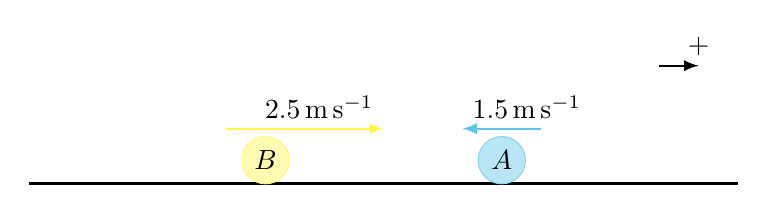
\begin{tikzpicture}
	\begin{scope}
	\draw [very thick] (-5,0)--(4,0);
	\draw [fill = b1!30,draw = b1!50] (1,0.3) circle (0.3) node{$A$};
	\draw [-latex,b1!70,thick] (1.5,0.7) -- (0.5,0.7) node[above right,black] {\SI{1.5}{\metre\per\second}};
	\draw [fill = yellow!30,draw = yellow!50] (-2,0.3) circle (0.3) node{$B$};
	\draw [-latex,yellow!70,thick] (-2.5,0.7) -- (-0.5,0.7) node[above left,black] {\SI{2.5}{\metre\per\second}};
	\draw [-latex,thick] (3,1.5) -- (3.5,1.5) node[above]{+};
	%\node at (1.5,0.375) {$A$};
	%\node at (-2.5,0.375){$B$};
	\end{scope}
\end{tikzpicture}

\end{document}